% Search for all the places that say "PUT SOMETHING HERE".


\documentclass[11pt]{article}
\usepackage{amsmath,textcomp,amssymb,geometry,graphicx,tkz-graph, qtree}

\def\Name{Ben Augarten}  % Your name
\def\Sec{106}  % Your discussion section
\def\Login{cs170-bo} % Your login

\def\pm{\begin{pmatrix}}
\def\epm{\end{pmatrix}}

\title{CS170--Fall 2012 --- Solutions to Homework 8}
\author{\Name, section \Sec, \texttt{\Login}}
\markboth{CS170--Spring 2012 Homework 8 \Name, section \Sec}{CS170--Spring 2012 Homework 8 \Name, section \Sec, \texttt{\Login}}
\pagestyle{myheadings}

\begin{document}
\maketitle
\begin{enumerate}
\item The Garage Sale Problem. This is almost exactly like the traveling salesman problem except we are trying to maximize the benefit minus transportation rather than minimize transportation. We can use the same subproblem however, because it involves essentially the same logic. The only difference is that we don't necessarily have to include every garage sale. Assuming we have a subset of garage sales $S=\{1,2,..,n\}$, all of which we have either visited or chosen to skip that include $1$ and $j\in S$ and ends at $j$, let $B(S,j)$ be the maximum possible benefit of visiting any arbitrary subset of garage sales in $S$ exactly once, starting at $1$ and ending at $j$. We define $B(S,1)$ for $|S|>1$ to be $0$ since there is no benefit of staying at home. Now we can find the previous garage sale we were at using this subproblem: $B(S,j)=\max_{i\in S, i\neq j} \{B(S-\{j\},i)+v_j-d_{ij}\}$ or we don't include it, and just add $j$ to the visited/skipped set: $B(S,i)=B(S-\{j\},i),\forall j\in S$\\, 
we either keep $j$ in the set, choosing not to visit it, or take the max with $j$ in the set along with the corresponding cost/reward. Note that $B(S,i)$ in the second case would just equal $B(S-\{j\},i)$ which we already knew.
The pseudocode is as follows:\\
\begin{verbatim}
C({1},1)=0
for s=2 to n:
  for all subsets S={1,2,..,n} of size s and containing 1:
    C(S,1) = 0
    for all j\in S, j\neq 1
      B(S,j),B(S,i)=max(B(S-{j},i)+v_j-d{ij}), max(B(S-\{j\},i)):i\in S, i\neq j)
return min_j B({1,..,n},j)+d_{j1}
\end{verbatim}
Correctness: Our update step and base case are correct, so the solution is! If we have a set of vertices that have been visited where the last one that was seen was $j$, then the maximum benefit of the subset either includes $j$ or doesn't include $j$. If it doesn't include $j$ then the maximum benefit is that of $j's$ parent. If it does, then its the benefit of the parent minus the distance to $j$ plus the benefit.\\
Runtime: We didn't change the number of subproblems, so there are $2^n*n$ subproblems, each of which still takes $n$ time to solve because we only have to loop through all of the $i$'s once, so it still takes $O(n^22^n)$ 
\newpage
\item
Expected search cost is $\sum_{i=1}^{n}\text{depth}(n_i+1)p_i=1+\sum_{i=0}^n\text{depth}(n_i)p_i$.\\
Obviously a tree is only optimal if its subtrees are optimal. So given $k$ keys, $n_1,..,n_k$ we assign the root to each $n_i$, and then recurse, finding the optimal substructure for each $n_1,..,n_{i-1}$ and $n_{i+1},..,n_k$ Of course, If there is only one element then the optimal substructure is just that element. So, we can formulate this recursively:
\begin{verbatim}
make_binary_tree(N={n_1,..,n_n},P={p_1,..,p_n})
if len(N) == 1: return n_1, p_1
trees = []
for n_i in {n_1,..,n_n}:
  extra-weight = p_i+sum(p_1,..,p_{k-1})
                 +sum(p_{k+1},..,p_n)
  left, cost_left = make_binary_tree({n_1,..,n_{k-1}},{p_1,..,p_{k-1}})
  right, cost_right = make_binary_tree({n_{k+1},..,n_n},{p_{k+1},..,p_n})
  trees.push((Tree(n_i,left=left,right=right), 
             cost_left + cost_right + extra-weight))
return the tree with the lowest cost
\end{verbatim}
Essentially, for each tree, choose each key as a root. If it has the lowest expected cost (where the cost is computed recursively in the subtrees and then add the frequencies for each level down the tree they go) then return it. Also note that we need to save the cost calculations, which I didn't show in the pseudocode out of laziness, but really we should store cost[1,..,i-1]=cost\_left and cost[i+1,..,n]=cost\_right, but this makes the code messier because then we have to use make our subscripts consistent (which I didn't do)\\
Correctness: We try each root, each subtree for each root is optimal, so the subtree with that root would be the optimal tree with that root. One of these has to be the optimal tree since we try all roots, so it must be correct.\\
Runtime: For each root we have to compute the left and right subtree. This amounts to doing $n^2$ work for each root, so its $O(n^3)$
\newpage
\item 
\begin{enumerate}
\item We can order the computations of edit distance such that we can reuse memory allocated for the matrix. First go all the way down the row of the matrix. Now we have every value in the first row. Using these values, we can calculate all of the values in the second row. We note that with any row in the matrix, we can calculate the next row. Therefore, we only need to keep one row in memory at a time, along with the next row that we are calculating. This uses $O(n)$ space.
\item When we get to the $m/2^{th}$ row, we have to start keeping track of a new value, at which $k$ we should halve the second string to produce the optimal edit distance. So at the $m/2^{th}$ row, we label $H(m/2,j)=j$ (H is going to keep track of the ending index of the second string we should pair with the first half of the first string to have the optimal edit distance, so $H(m,n)$ at the end of the algorithm will hold $k$).\\
So now the question is how to get the next row of $H$ given the row at $m/2$. We can get the next row by noting that after the $m/2^{th}$ row, $H(i,j)=H(i-1,j)$ if $Edit(i,j)=Edit(i-1,j)+1, H(i,j)=H(i,j-1)$ if $Edit(i,j)=Edit(i,j-1)+1$, and $H(i,j)=H(i-1,j-1)$ otherwise. That is, if we got the $i,j$ edit distance from inserting a letter, then we should use the half that we got from that path, or if we got the $i,j$ edit distance from deleting  letter, then we should use that half, or if it was a substitution we should use that $k$ value. We can compute each row of $H$ from the previous, so $O(n+m)$ space.

\item We can calculate the $k$ in $O(nm)$ time and linear space. \\
$T(n,m)=T(n/2,k)+T(n/2,m-k)+O(nm)$\\
We can approximate it with: $T(n,m)=2T(n/2,m/2)+O(nm)$\\
$=2^2T(n/2^2,m/2^2)+(mn/2)+mn$\\
$=2^3*T(n/2^3,m/2^3)+mn/2^2+mn/2+mn$\\
$=2^iT(n/2^i,m/2^i)+mn/2^{i-1}+..+mn/2+mn$\\
$=mn/2^{\log_2(n)}+..+mn/2+mn$\\
$=O(mn)$\\
So its $O(mn)$ runtime and by a similar argument (the size of the problem decreases by a factor of $2$ each time), the space requirement is dominated by the first iteration so it takes $O(n+m)$ space.

\end{enumerate}
\newpage
\item
\begin{enumerate}
\item[7.1]
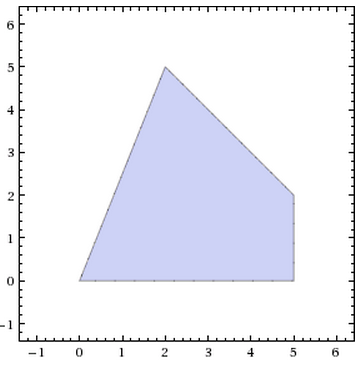
\includegraphics[width=200px]{graph.png}\\
We maximize $5x+3y$ in the feasible region, so the maximum is at $(5,2)$
\item[7.2] Let $a$ be the number of shnupells of duckwheat produced in Mexico and sent to NY, \\
$b$ the number made in Mexico and sent to CA, \\
$c$ the number produced in Kansas and sent to NY, \\
$d$ the number produced in Kansas and sent to NY.\\
\\
minimize \\
$4a+b+2c+3d$\\
constraints: \\
$c+d = 15$, Kanasas produces 15\\
$a+b=8$, Mex produces 8\\
$a+c=10$, NY consumes 10\\
$b+d=13$, CA consumed 13\\
\end{enumerate}
\end{enumerate}
\end{document}
